% Chapter 3

\chapter{Results} % Main chapter title
\label{Chapter3} % For referencing the chapter elsewhere, use \ref{Chapter3} 
\addtocontents{toc}{\setcounter{tocdepth}{1}}
\section{Assessment of inducible GLUT1 expression}
Previous results from the work of our laboratory showed that the GLUT1\textsuperscript{P485L} mutation leads to specific interaction with clathrin and the internalization of the protein. In order to further investigate the role and functional effects of the mutation, we used two Flp-In T-Rex HEK293 cell lines containing inducible BirA-FLAG epitope-tagged full length wild-type or mutant GLUT1 (Figure~\ref{fig:vectors}). The cells constitutively express Tet repressor (TetR) which binds to the TetO\textsubscript{2} sequence in the promoter of transgenic GLUT1~\cite{Hillen}. Upon addition, tetracycline binds to the TetR, causing the release of TetR from TetO\textsubscript{2} and induction of transgene transcription~\cite{Hillen}. In this thesis doxycycline was used as a relatively stable tetracycline derivative to induce the expression of the BirA-FLAG tagged GLUT1 variants~\cite{Xu}.

To determine the optimal conditions for inducible expression, GLUT1 wild-type and mutant cells were grown in different concentrations of doxycycline for 24 hr and the expression of the GLUT1 protein was analyzed by Western blotting with an anti-FLAG antibody. No GLUT1 expression was detected in the absence of doxycycline (Figure~\ref{fig:wb} A). Compared with 0.1 \textmu g/mL doxycycline, induction with 1 \textmu g/mL doxycycline resulted in higher GLUT1 levels in wild-type cells, whereas in mutant cells the GLUT1 expression was not significantly altered (Figure~\ref{fig:wb} A and C). The results showed that the lower dose of doxycycline was sufficient for induction of the system. 

Additionally, GLUT1 protein expression was quantified after 24 hr and 48 hr of doxycycline induction. Further increase in the induction time did not result in increased GLUT1 levels in wild-type cells, but actually decreased the expression in mutant cells compared to the 24 hr time point (Figure~\ref{fig:wb} B and D). Therefore the induction with 0.1 \textmu g/mL doxycycline for 24 hr was selected in the following experiments to reduce toxic side effects of the drug~\cite{Zeltser}.

\begin{figure}[h]
\centering
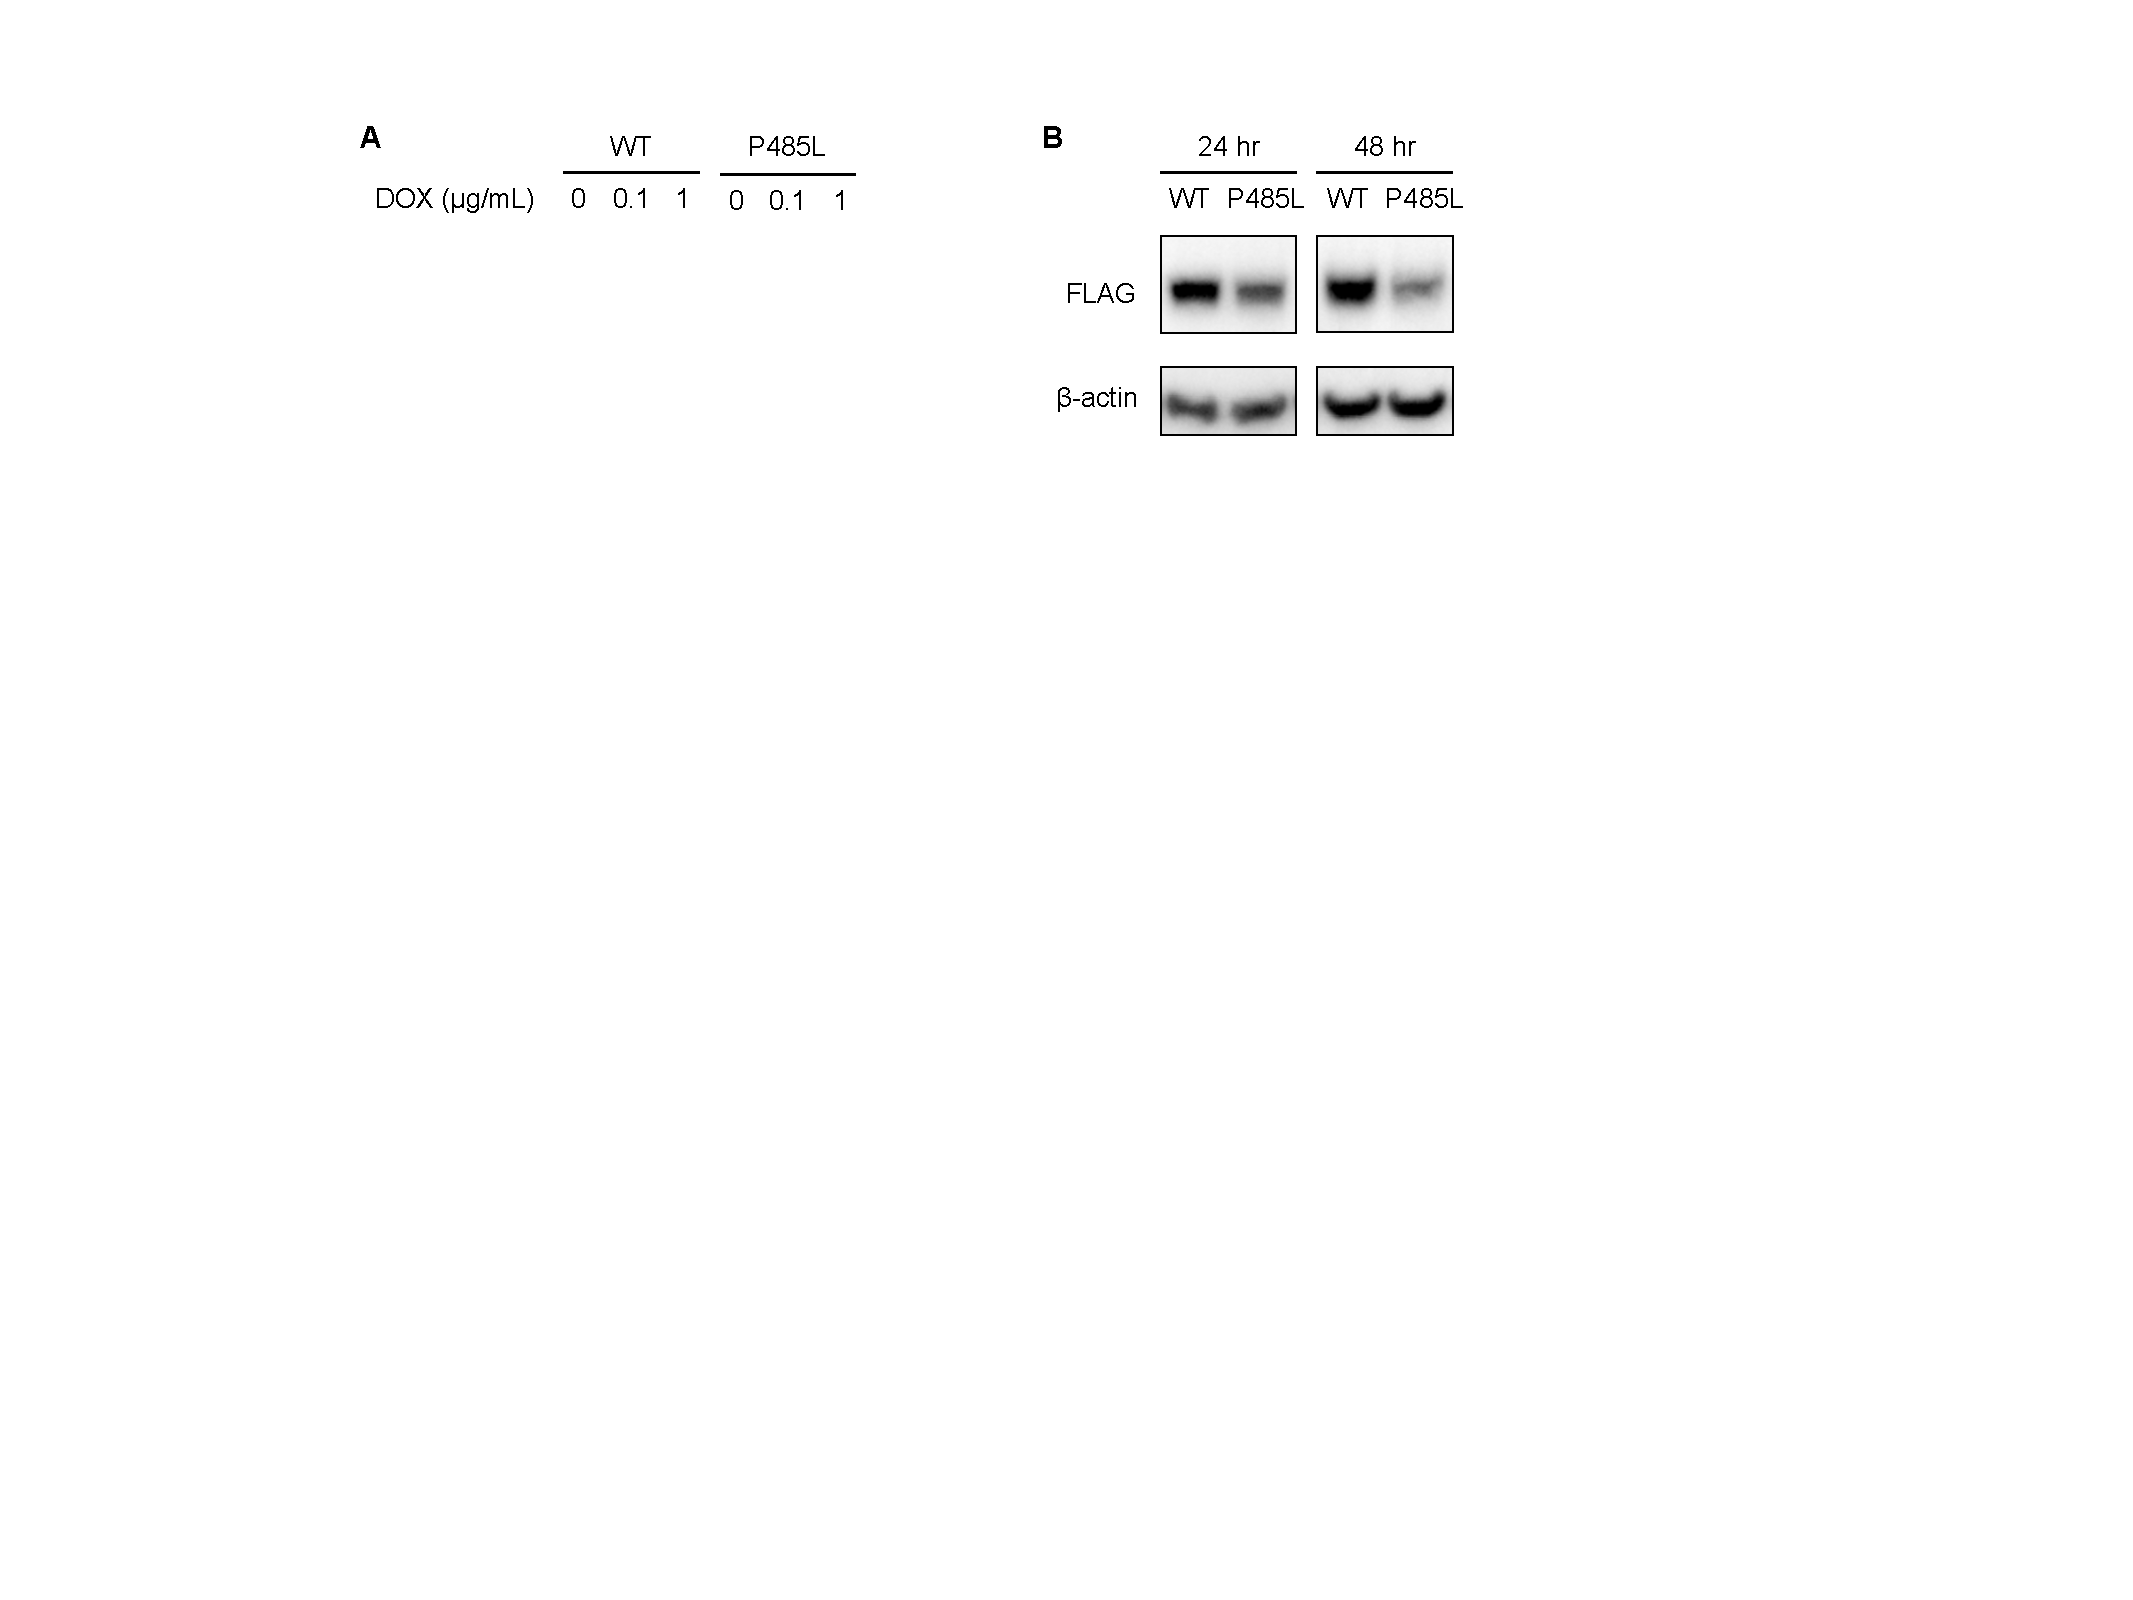
\includegraphics[scale=0.7]{Figures/WB}
\caption{The doxycycline-inducible expression of GLUT1 variants.}
%\smallskip
\vspace*{-3mm}
\small \justify
Different conditions were investigated to induce the expression of BirA-FLAG tagged GLUT1 with doxycycline. GLUT1 wild-type (WT) and mutant (P485L) cells were treated with varying concentrations of doxycycline (0, 0.1 or 1 \textmu g/mL) for 24 hr and analyzed with Western blotting (A). The inducible expression of GLUT1 was also compared between 24 hr and 48 hr induction with 0.1 \textmu g/mL doxycycline (B). Quantification of GLUT1 levels was achieved by normalizing to \textbeta -actin (C, D).
\label{fig:wb}
\end{figure}
Furthermore, the doxycycline-inducible expression of GLUT1 was confirmed by immunofluorescence confocal microscopy. A different anti-FLAG antibody (see "Methods" section) was used to analyze transgene expression with or without doxycycline treatment in both cell lines. Interestingly, although leakiness in expression was not detected in Western blotting, a small subpopulation of uninduced wild-type and mutant cells showed transgene expression in immunofluorescence microscopy (Figure~\ref{fig:if} A and B), 
% In addition, a low basal expression of FLAG-tagged GLUT1 was visible under stronger laser excitation in uninduced wild-type cells, Supplementary fig???, 
suggesting the existence of leaky expression from the Tet promoter in the absence of doxycycline~\cite{Pham,Senkel}. 
In consistence with Western blotting results, strong and roughly uniform expression in response to doxycycline was observed in wild-type and mutant cells (Figure~\ref{fig:if} C and D). 
\begin{figure}[h]
\centering
\includegraphics[scale=0.7]{Figures/if}
\caption{The inducible expression of GLUT1 variants assessed by immunofluorescence microscopy.}
\vspace*{-3mm}
\small \justify
GLUT1 wild-type (WT) and mutant (P485L) cells were cultured on coverslips for 24 hr either in the absence (A, B) or presence (C, D) of 0.1 {}\textmu g/mL doxycycline. Immunostaining of BirA-FLAG tagged GLUT1 was performed with monoclonal mouse anti-FLAG and Alexa 488-conjugated anti-mouse antibodies (green). Cell nuclei were identified by DAPI staining (blue). Scale = 10 \textmu m.
\label{fig:if}
\end{figure}
%As expected, ARF localized to nucleolar regions (the compact circular regions of higher intensity as pointed by the arrow in panel A) while HA-RBP1 demonstrated strong nuclear localization with nucleolar exclusion, as shown by the dark nucleolar regions in panel B. Panel C confirms that RBP2 is localized exclusively to the nucleus. Panel D illustrates that the rabbit polyclonal ?-RBP2 antibody cannot be used in immunofluorescence because of the high amount of non-specific background signal it produces. Trials were done at various dilutions but all were negative and produced the same non-specific noise (data not shown). 

\section{Effect of blocking proteolysis on GLUT1 levels}
Despite the approximately uniform expression within both cell lines, a lower level of GLUT1 expression was observed in mutant cells than in wild-type cells (Figure~\ref{fig:wb}). We thus speculated that the mutant protein might undergo degradation through proteolytic pathways. A rescue experiment was designed to determine the effect of proteolysis on GLUT1 levels by using proteolytic inhibitors Bafilomycin A1 or MG132 to block lysosomal degradation or proteosomal degradation, respectively~\cite{Tanida,Lee.2}. The GLUT1 levels in cells with or without inhibitor treatment were quantified by Western blotting analyses.
%(Figure~\ref{fig:wb2}). 

Bafilomycin A1 inhibits the vacuolar type H\textsuperscript{+}-ATPase complex necessary for lysosomal acidification, thus blocks protein degradation in lysosomes~\cite{Yamamoto,Klionsky}. The inhibitory effect of Bafilomycin A1 was confirmed by the accumulation of LC3-phosphatidylethanolamine conjugate (LC3-II) upon inhibitor treatment (Figure~\ref{fig:wb2} A). Surprisingly, the inhibition decreased wild-type GLUT1 levels by approximately 10\% in comparison to the untreated control group, whereas in mutant cells the inhibition increased GLUT1 levels by around 30\% (Figure~\ref{fig:wb2} B). These results suggest that lysosomal degradation might be partially responsible for the differential GLUT1 protein levels in the two cell lines, but independent sets of experiments and quantification need to be repeated.

\begin{figure}[h]
\centering
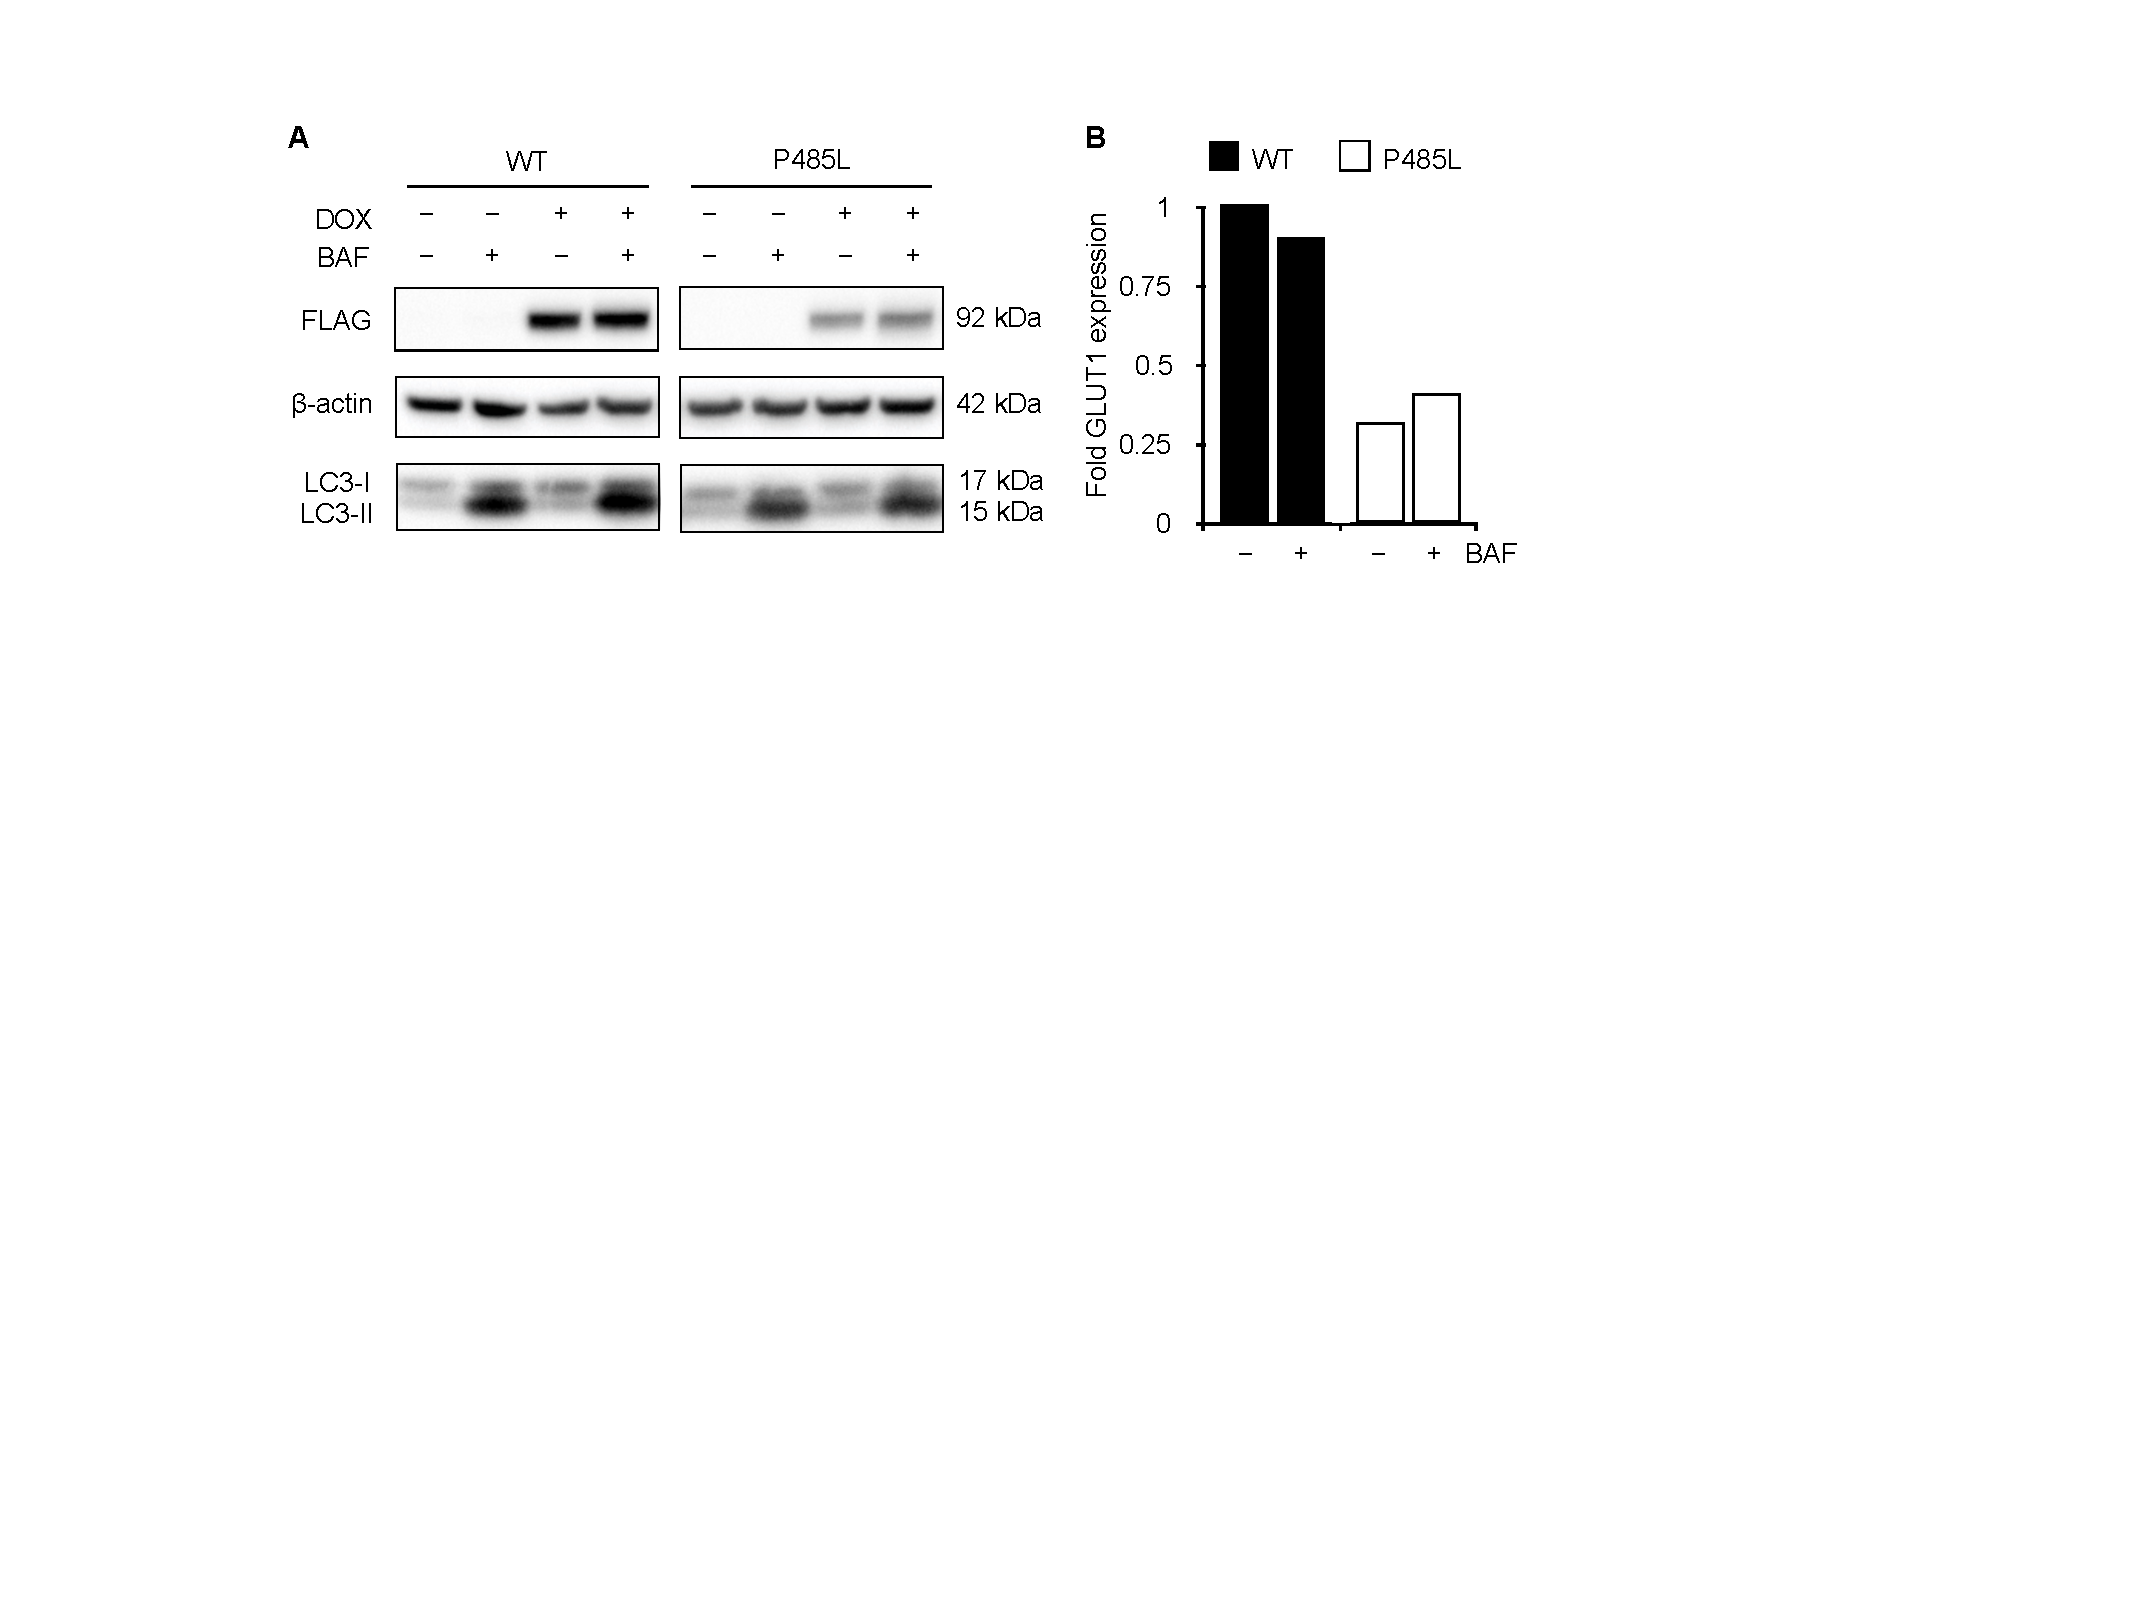
\includegraphics[scale=0.7]{Figures/wb2}
\caption{The effect of blocking lysosomal degradation on GLUT1 levels.}
\vspace*{-3mm}
\small \justify
GLUT1 wild-type (WT) and mutant (P485L) cells were incubated in 0.1 \textmu g/mL doxycycline for 18 hr before Bafilomycin A1 (BAF, final concentration: 250 nM) or carrier control (DMSO) was added. After 6 hr of drug treatment, the cells were lysed and the GLUT1 levels were analyzed in Western blotting (A). Quantification of GLUT1 levels in induced cells was achieved by normalizing to \textbeta -actin (B).
\label{fig:wb2}
\end{figure}
To demonstrate that the proteosomal inhibitor MG132 did decrease proteosomal degradation, cells were transfected with HA epitope-tagged UL21a after doxycycline induction. UL21a has been reported to encode the viral protein pUL21a, a short-lived cytoplasmic protein targeted for proteosome-dependent degradation and can be drastically stabilized in the presence of MG132~\cite{Fehr}. The cells were treated with MG132 or DMSO control after UL21a transfection, and analyzed for the accumulation of HA-tagged pUL21a and FLAG-tagged GLUT1 levels by Western blotting. The accumulation of pUL21a was observed after MG132 treatment, but no significant effect of proteosomal inhibition was shown on wild-type and mutant GLUT1 levels (Figure~\ref{fig:wb3}).

\begin{figure}[h]
\centering
\includegraphics[scale=0.7]{Figures/wb3}
\caption{The effect of blocking proteosomal degradation on GLUT1 levels.}
\vspace*{-3mm}
\small \justify
GLUT1 wild-type (WT) and mutant (P485L) cells were incubated in 0.1 \textmu g/mL doxycycline for 1 hr before being transfected with HA-UL21a. At 17 hr after transfection, MG132 (final concentration: 20 mM) or DMSO control. Cells lysates were collected 6 hr later and analyzed by immunoblotting with an anti-FLAG antibody to determine GLUT1 levels and an anti-HA antibody for pUL21a levels (A). The GLUT1 level in doxycycline induced cells were quantified by normalizing to \textbeta -actin (B).
\label{fig:wb3}
\end{figure}
%we examined LC3-II or p62 levels in serum-starved cellseither in the absence, or presence of bafilomycin A1, an agent thatinhibits lysosomal acidification and/or inhibits autophagosome-lysosome fusion; this treatment leads to reduced degradation andhence, accumulation of autophagy substrates A Role for Presenilins in Autophagy Revisited: Normal Acidification of Lysosomes in Cells Lacking PSEN1 and PSEN2 (PDF Download Available). Available from: https://www.researchgate.net/publication/227858130_A_Role_for_Presenilins_in_Autophagy_Revisited_Normal_Acidification_of_Lysosomes_in_Cells_Lacking_PSEN1_and_PSEN2 [accessed Jul 13, 2017].
%LC3-II levels were elevated in cultured WT-ES cells(Fig. 1A, compare lanes 1, 2)
\section{Cellular localization of GLUT1 variants}
The plasma membrane localization of wild-type GLUT1 has been well demonstrated in sequence and structure-based studies~\cite{Mueckler.2,Hresko,Hruz}.
To compare the localization of wild-type and mutant GLUT1, we examined the localization in the two stable cell lines by immunofluorescent microscopy. Expression of the FLAG-tagged wild-type GLUT1 was clearly detected on the cell surface (Figure~\ref{fig:glut1} B). Conversely, the FLAG-tagged mutant GLUT1 was mostly localized in intracellular regions (Figure~\ref{fig:glut1} D). Additionally, this differential localization was confirmed by using an anti-GLUT1 antibody (Figure~\ref{fig:glut1} A and C).

\begin{figure}[h]
\centering
\includegraphics[scale=0.7]{Figures/glut1}
\caption{The differential cellular localization of GLUT1 variants.}
\vspace*{-3mm}
\small \justify
Localization of GLUT1 wild-type (WT) and mutant (P485L) was analyzed in HEK293 cells induced with 0.1 \textmu g/mL doxycycline for 24 hr. Immunostaining of the FLAG-tagged GLUT1 variants was performed with rabbit anti-GLUT1 and Alexa 488-conjugated anti-rabbit antibodies (green, A and D), as well as mouse anti-FLAG and Alexa 568-conjugated anti-mouse antibodies (red, B and E). The overlay images with DAPI-stained nuclei were also shown (C and F). Scale = 10 \textmu m.
\label{fig:glut1}
\end{figure}
\section{Proximity labeling of GLUT1 variants}
In order to systematically characterize the subcellular localization of the wild-type and mutant GLUT1, proximity-dependent biotinylation (BioID) was used to label neighboring proteins within approximately 20 nm of the BirA-tagged GLUT1 variants~\cite{Kim,Dong}. Three-state stable isotope labeling with amino acids in cell culture (SILAC) in combination with mass spectrometry analysis was used to quantitatively identify the \textit{in situ} biotinylated proteins. A HEK293 stable cell line containing the GFP1-10 transgene was used as nonbiotinylated negative control in the light channel (Figure~\ref{fig:bioid}). 

Consistent with microscopy results shown in Figure~\ref{fig:glut1}, many of the specific proximal proteins of the wild-type GLUT1 are either transmembrane proteins on the cell surface, such as members of the SLC superfamily (SLC4A7, SLC1A5 etc), or cytosolic proteins that peripherally associate with transmembrane proteins, such as ephrin ligands (EFNB1, EFNB2) (Figure~\ref{fig:bioid2})~\cite{He,Himanen}. 
\begin{figure}[h]
\centering
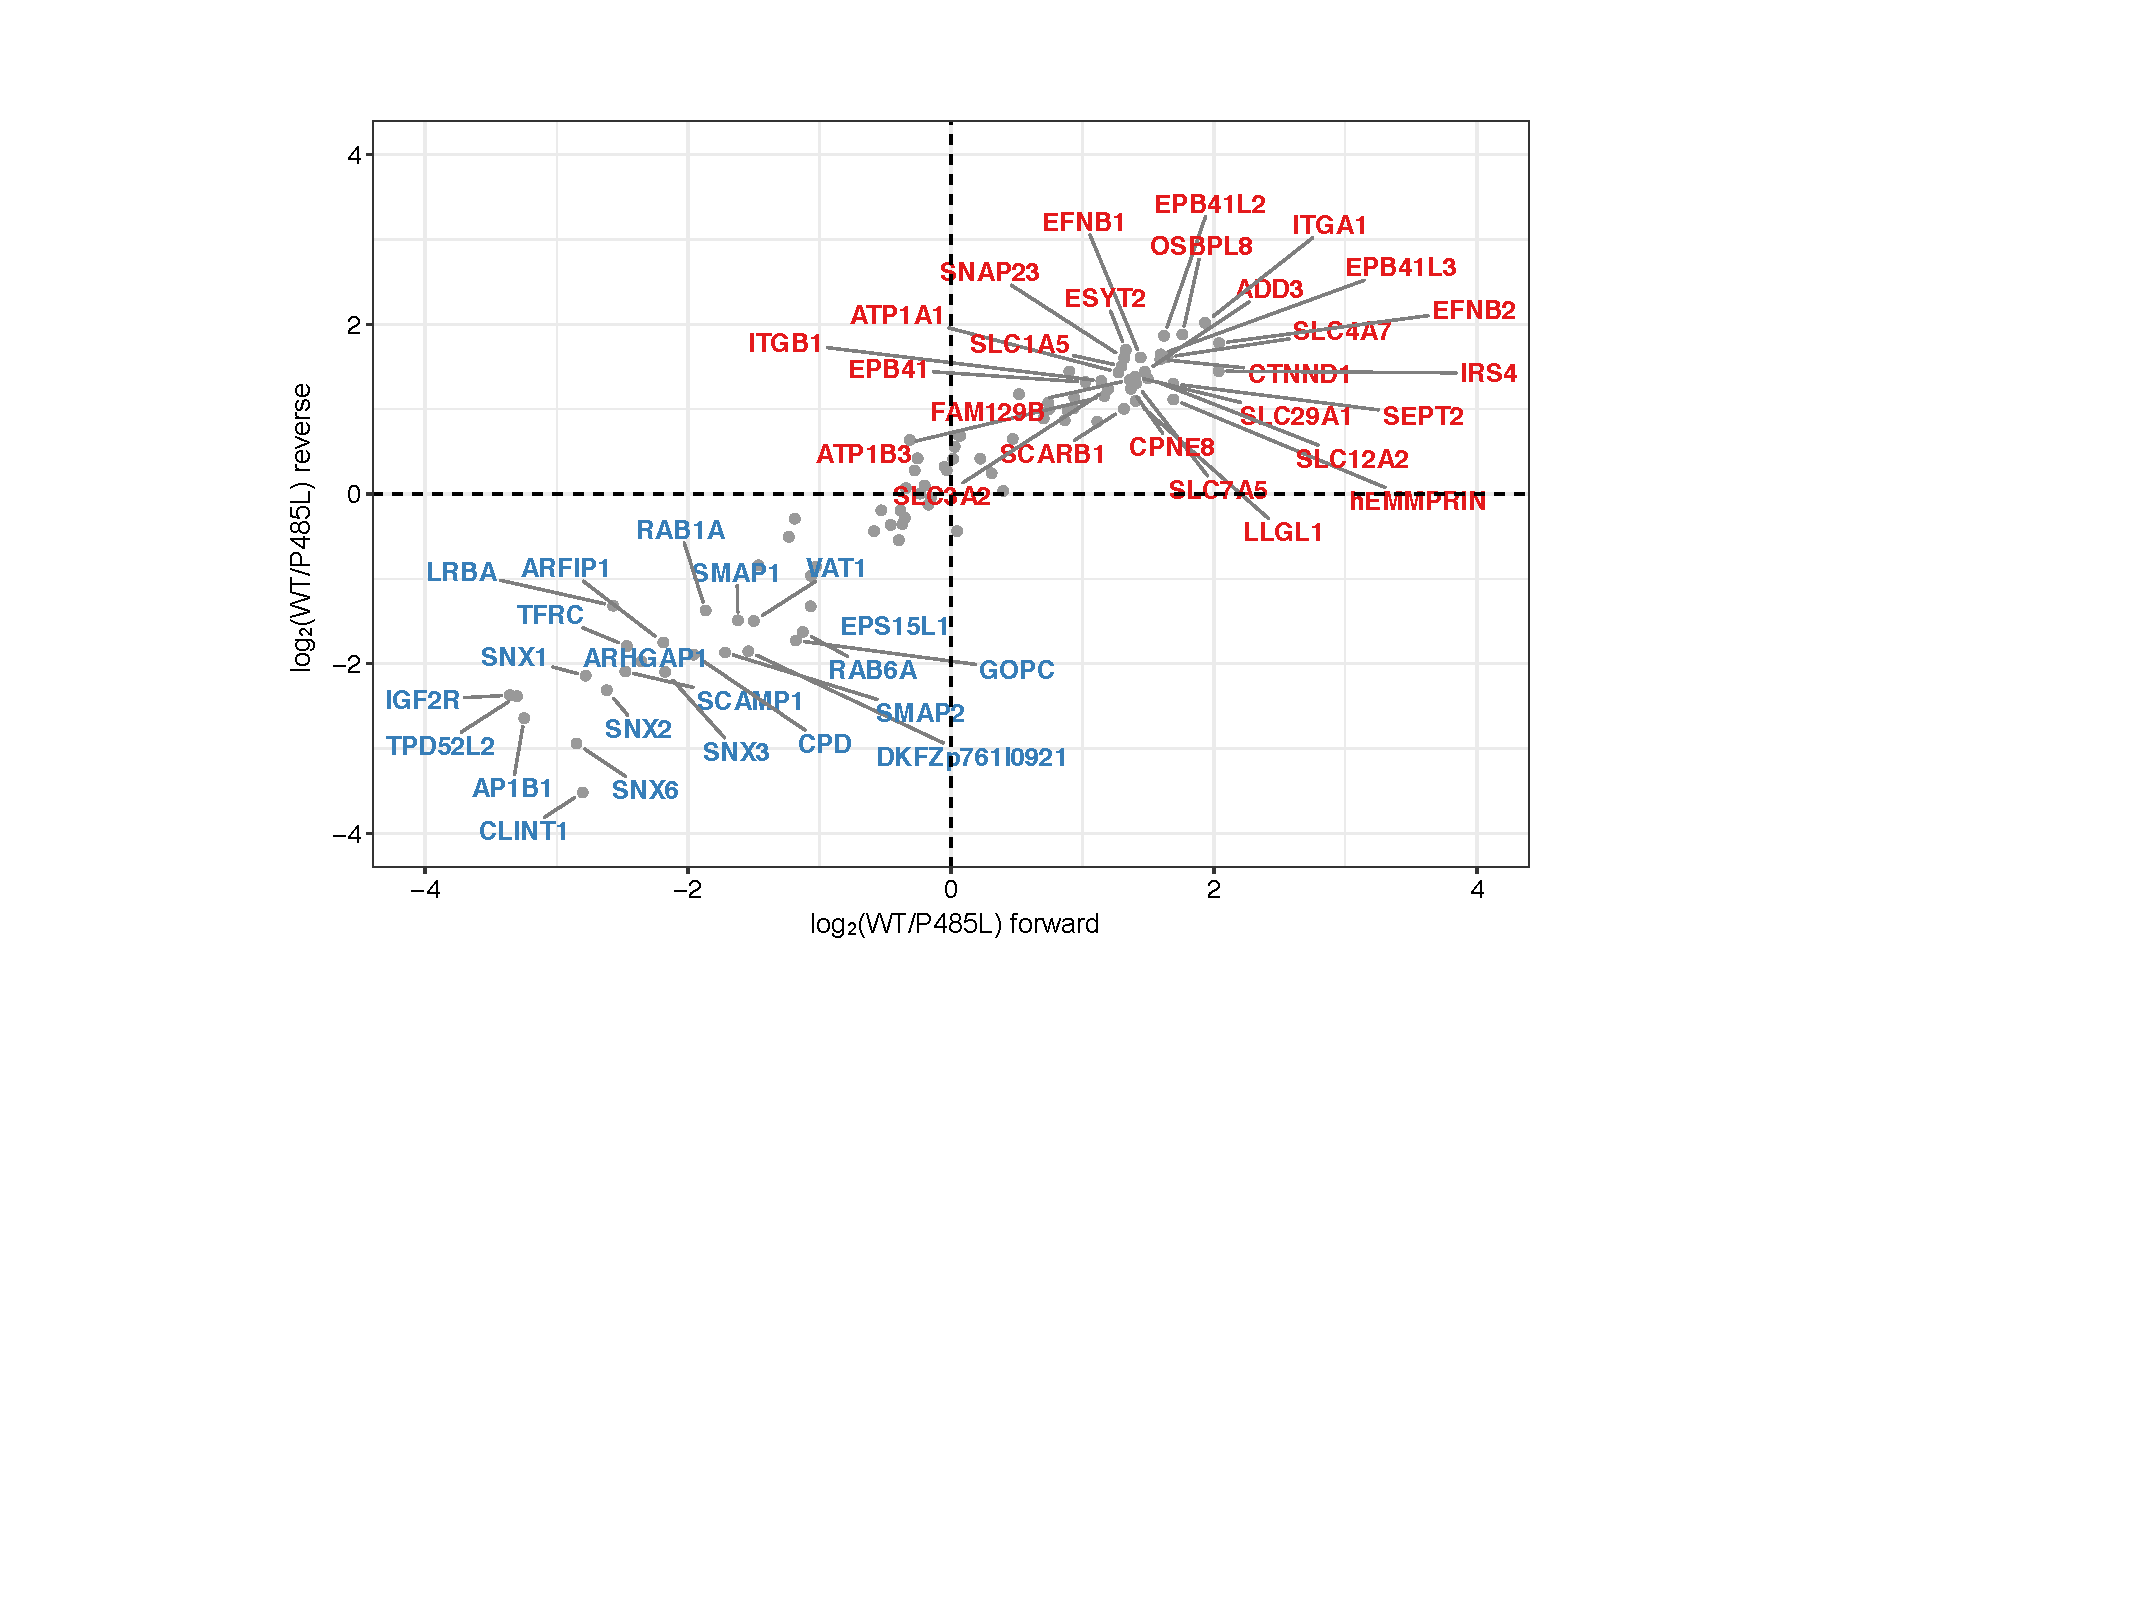
\includegraphics[scale=0.7]{Figures/bioid2}
\caption{SILAC ratio of proteins proximal to the GLUT1 variants.}
\vspace*{-3mm}
\small \justify
HEK293 stable cells expressing GFP1-10 were fully labeled in light (L) isotope medium, whereas HEK293 stable cells expressing BirA-FLAG-GLUT1 wild-type (WT) and BirA-FLAG-GLUT1 mutant (P485L) were fully labeled in medium-heavy (M) or heavy (H) isotope media. The cells were incubated in 0.1 \textmu g/mL doxycycline and 1 mM biotin for 24 hr before being harvested. Purified proteins were quantified by MS/MS analysis. Proteins with a SILAC heavy/light (H/L) or medium/light (M/L) ratio smaller than 1.5 were considered to be background proteins and discarded. After background subtraction, proteins with a SILAC wild-type/mutant (WT/P485L) ratio or mutant/wild-type (P485/L) higher than 2 in both forward and reverse experiments were identified as specific proximal proteins and the gene names were annotated.
\label{fig:bioid2}
\end{figure}

%Moreover, some of the other proteins identified to be proximal to wild-type GLUT1 have been reported
Conversely, many proteins involved in intracellular trafficking were identified to be proximal to the mutant GLUT1 (Figure~\ref{fig:bioid2}), including sorting nexins (SNX1, SNX2, SNX3) which are components of the retromer complex mediating the retrograde transport from endosomes to the trans-Golgi network~\cite{Rojas,Carlton,Mari,Harterink}. CLINT1, the protein with high mutant/wild-type ratios in both forward and reverse experiments, has been suggested to participate in the transport of cargo proteins via clathrin-coated vesicles from the trans-Golgi network to endosomes~\cite{Mills,Kalthoff,Hirst}. Moreover, IGF2R and TRFC, two receptors identified as proximal proteins of the mutant GLUT1, have been reported to mediate the intracellular trafficking of their corresponding ligands via clathrin-coated vesicles. IGF2R transports lysosomal enzymes from the trans-Golgi network and the cell surface to lysosomes, whereas TRFC is responsible for the internalization of transferrin and its recycling back to the cell surface~\cite{Byrd,Daro}. 
% Together, these data confirmed the differential localization of the wild-type and mutant GLUT1 observed in immunofluorescence microscopy and further indicated that the mutant GLUT1 might reside in clathrin-coated vesicles, several endosomal compartments and the trans-Golgi network.
%At steady state, GLUT1 is localized at the plasma membrane from where it undergoes continuous rounds of endocytosis and PDZ-motif-dependent endosome-to-plasma-membrane recycling (Wieman et al., 2009), the latter being mediated by the SNX27?retromer (Steinberg et al., 2013). RNA interference (RNAi)-mediated suppression of SNX27 or the retromer CSC component VPS35 leads to a pronounced decrease in the amount of GLUT1 at the cell surface and a corresponding decrease in whole-cell levels, as the transporter undergoes missorting and enhanced degradation in the lysosome (Steinberg et al., 2013).

\begin{figure}[h]
\centering
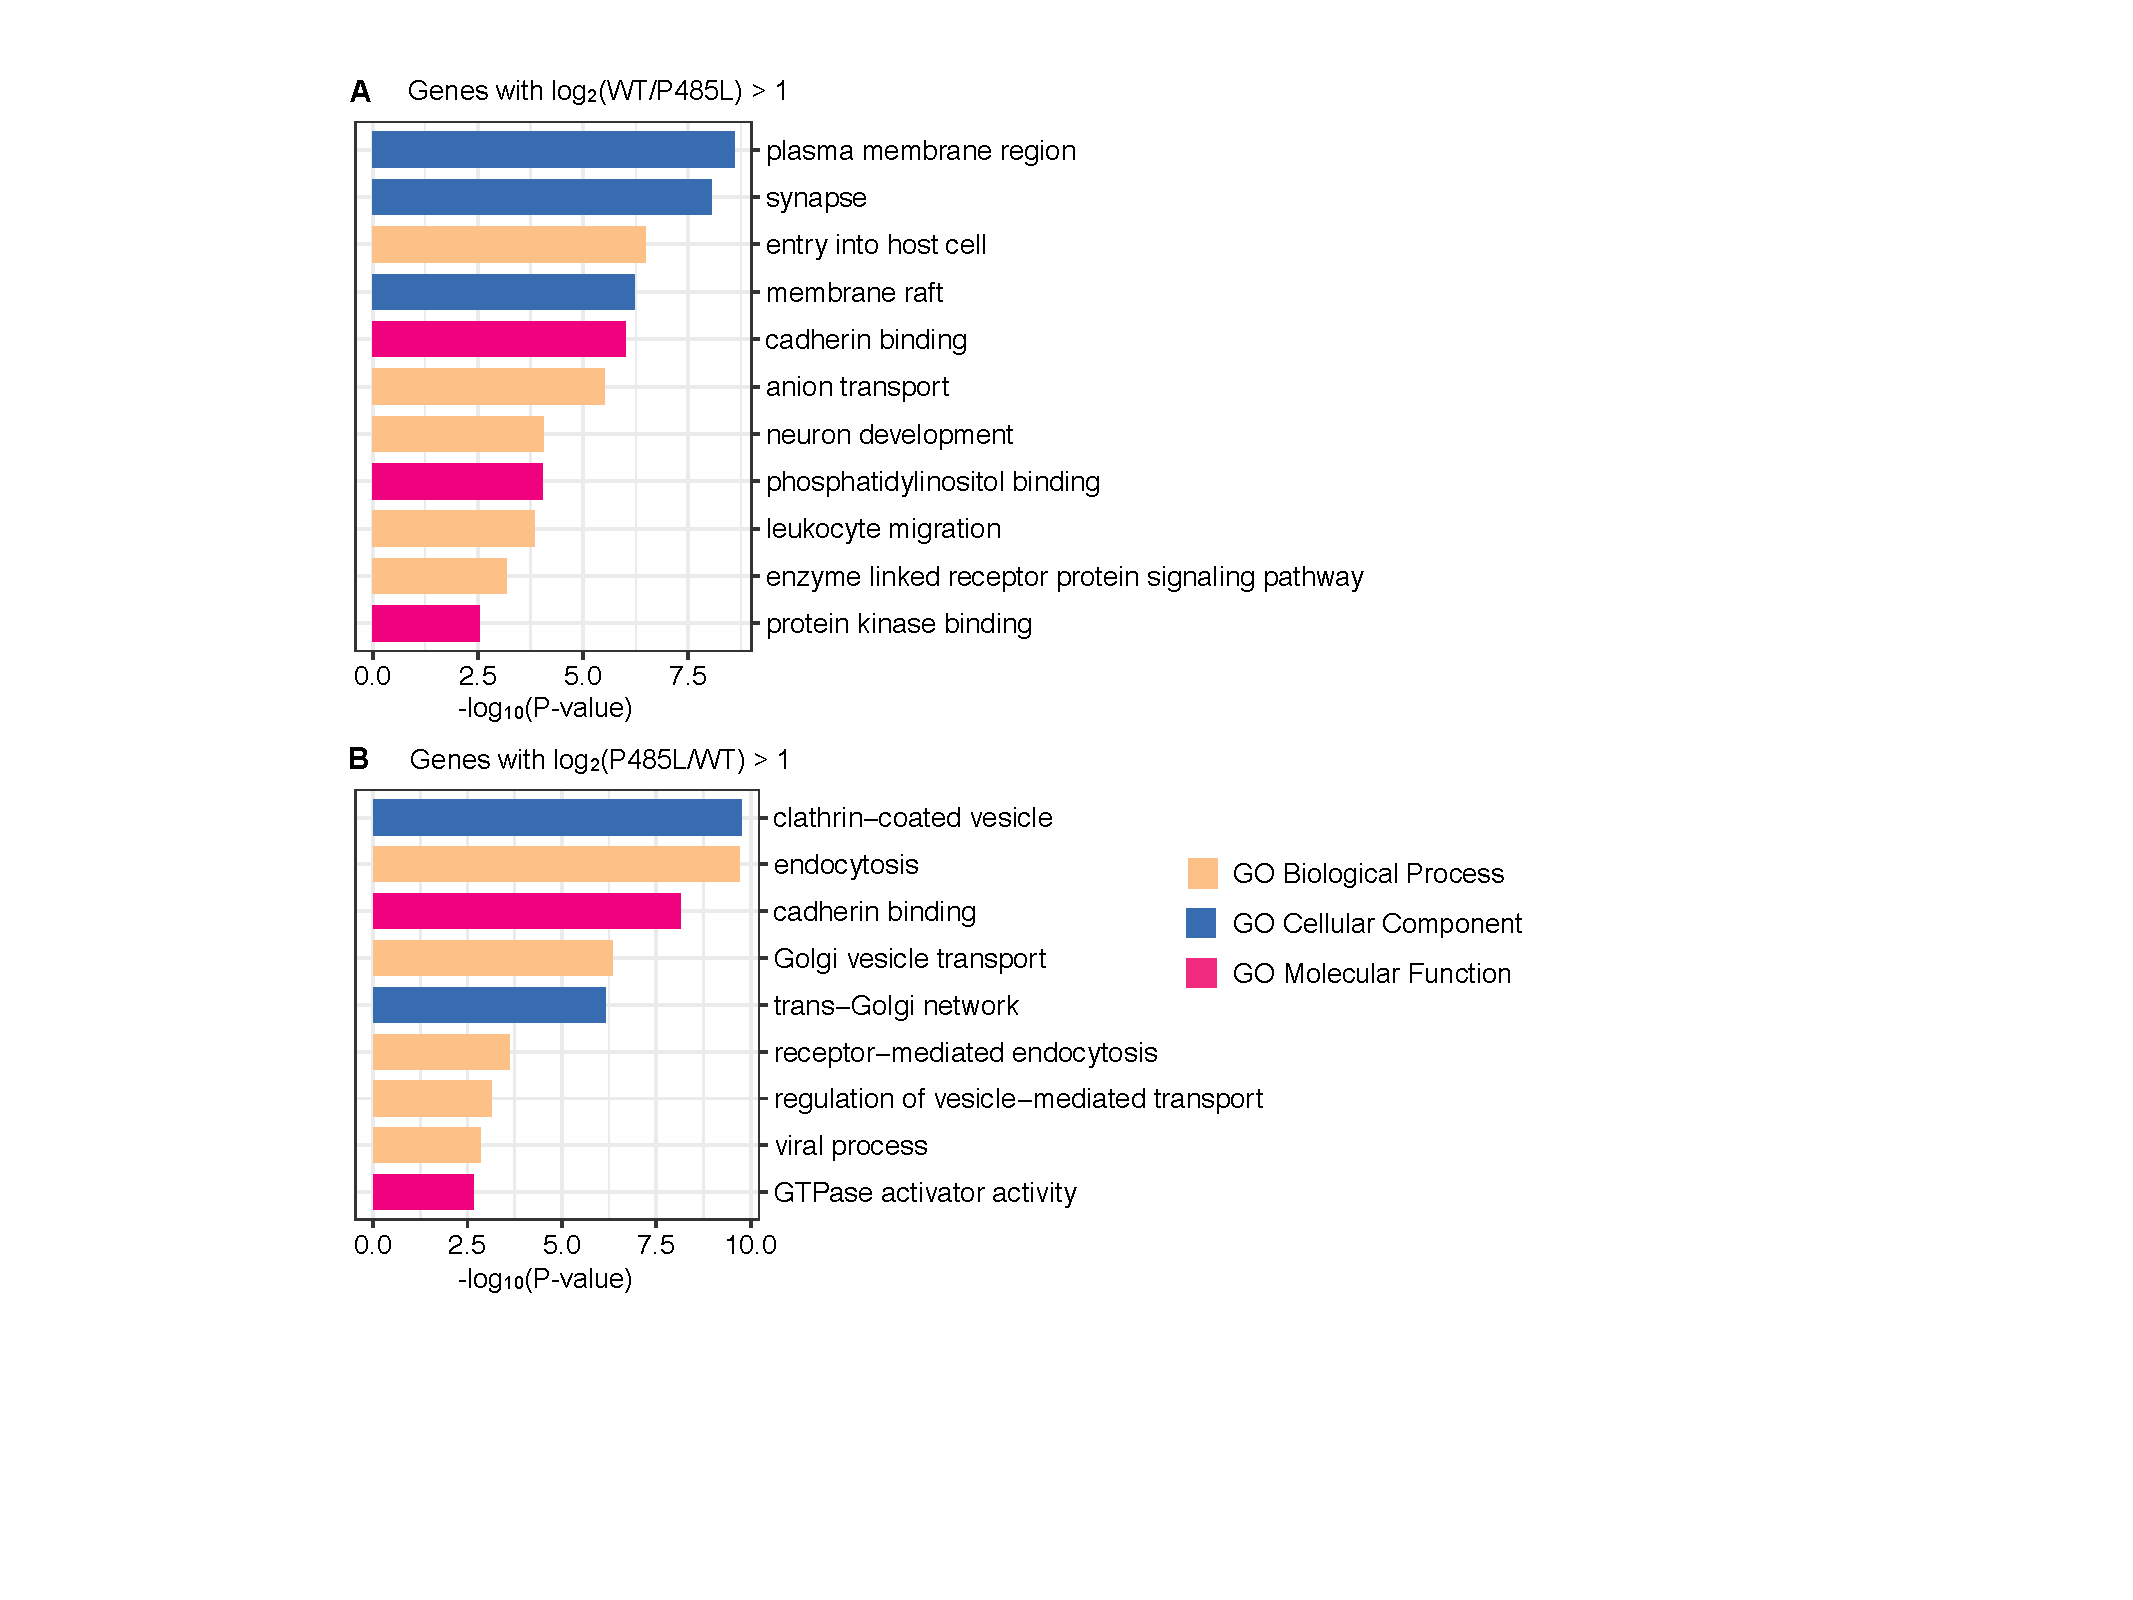
\includegraphics[scale=0.7]{Figures/GO}
\caption{Gene ontology enrichment analysis of GLUT1-proximal proteins.}
\vspace*{-3mm}
\small \justify
Gene ontology analysis was performed with Metascape~\cite{Tripathi}. Only proteins with SILAC H/L and M/L ratios larger than 1.5, WT/P485L ratios larger than 2 in both forward and reverse experiments were selected for the analysis of wild-type specific proteins (A); the analysis of mutant-specific proteins (B) only included proteins with SILAC H/L and M/L ratios larger than 1.5, P485L/WT ratios larger than 2.
\label{fig:go}
\end{figure}
Furthermore, gene ontology (cellular component) analysis of the annotated proteins in Figure~\ref{fig:bioid2} also showed that proteins colocalizing with the wild-type GLUT1 were enriched for plasma membrane proteins ($P=5.89\times 10^{-9}$). In contrast, proteins colocalizing with the mutant GLUT1 were more associated with clathrin-coated vesicles ($P=6.17\times 10^{-10}$), endosomes ($P=2.14\times 10^{-7}$) and retromer complexes ($P=2.45\times 10^{-7}$) (Figure~\ref{fig:go}). Endocytosis was also identified as a significantly enriched biological process in the proteins colocalizing with the mutant GLUT1 ($P=4.27\times 10^{-11}$).

Together, these data confirmed the differential localization of the wild-type and mutant GLUT1 observed in immunofluorescence microscopy and indicated that the P485L mutation in GLUT1 causes the internalization of the protein via clathrin-dependent endocytosis. Consequently, the mutant protein might reside in clathrin-coated endocytic vesicles, endosomal compartments and the trans-Golgi network.
\section{Co-localization study of GLUT1 variants}
To confirm that the mutant GLUT1 is taken up via clathrin-mediated endocytosis, doxycycline-induced cells were incubated with fluorescently-labeled transferrin (Tf), a known marker for clathrin-mediated endocytosis, and immunostained with the antibody against FLAG~\cite{Hanover}. As expected, extensive colocalization of endocytosed transferrin was detected with the mutant GLUT1, but not with the wild-type GLUT1 (Figure~\ref{fig:tf} C and F).
\begin{figure}[h]
\centering
\includegraphics[scale=0.7]{Figures/tf}
\caption{The mutant GLUT1 co-localizes with endocytosed transferrin.}
\vspace*{-3mm}
\small \justify
Wild-type (WT) and mutant (P485L) GLUT1-expressing cells were cultured on coverslips and induced with 0.1 \textmu g/mL doxycycline for 24 hr. The cells were then incubated with Alexa 568-conjugated transferrin (red, shown in greyscale in B and E) for 10 min before being fixed. The GLUT1 was stained with mouse anti-FLAG and Alexa 488-conjugated anti-mouse antibodies (green, shown in greyscale in A and D). Yellow in the overlay channels (C and F) indicates colocalization of green and red staining. Scale = 10 \textmu m.
\label{fig:tf}
\end{figure}
\begin{figure}[h]
\centering
\includegraphics[scale=0.7]{Figures/EE}
\caption{A subset of the mutant GLUT1 colocalizes with early endosomal markers.}
\vspace*{-3mm}
\small \justify
Wild-type (WT, A-F) and mutant (P485L, G-L) GLUT1-expressing cells were induced with doxycycline and then stained for GLUT1 with mouse anti-FLAG and Alexa 488-conjugated anti-mouse antibodies (green). EEA1 (A-C, G-I) and Rab5 (D-F, J-L) were stained with their corresponding rabbit monoclonal antibodies (Table~\ref{tab:IF}) and Alexa 568-conjugated anti-rabbit antibodies (red). The Rab5 co-staining images were taken with zoom 3 and cropped into the size as shown. Scale = 10 \textmu m.
\label{fig:ee}
\end{figure}

To further determine the subcellular localization of the mutant GLUT1, the GLUT1 expressing cells were co-immunostained with antibodies against organelle-specific marker proteins, including markers for early endosomes, recycling endosomes, late endosomes and the trans-Golgi network. The wild-type GLUT1 showed no colocalization with EEA1 and Rab5, two markers for early endosomes (Figure~\ref{fig:ee} C and I)~\cite{Mu}. By contrast, extensive colocalization was observed between the mutant GLUT1 and the early endosomal markers (Figure~\ref{fig:ee} F and L). Rab5 is a small GTPase involved in the formation of clathrin-coated vesicles (CCV) at the plasma membrane, their subsequent fusion with early endosomes, and the fusion between early endosomes, whereas EEA1 is one of the effector proteins of Rab5 and is recruited selectively on the membrane of early endosomes~\cite{Christoforidis,Rubino,Ballmer}. Because the endocytic CCV is devoid of EEA1, the staining patterns produced by antibodies to EEA1 and Rab5 were not identical (Figure~\ref{fig:ee} B, E, H and K). 
%Some colocalization was observed between Rab5 and the mutant GLUT1, however, the images for this co-staining experiment was taken with a lower resolution than other images, thus were excluded for quantitative colocalization analysis.

\begin{figure}[h]
\centering
\includegraphics[scale=0.7]{Figures/re}
\caption{The mutant GLUT1 does not colocalize with recycling endosomal markers.}
\vspace*{-3mm}
\small \justify
Cells expressing FLAG-tagged wild-type (WT) and mutant (P485L) GLUT1 were co-immunostained with antibodies against FLAG (green) and recycling endosomal markers (red), namely Rab4 (A-C, G-I) and Rab11 (D-F, J-L). Scale = 10 \textmu m.
\label{fig:re}
\end{figure}
We then asked whether the mutant GLUT1 follows the same endosomal recycling as transferrin. Antibodies against two Rab proteins implicated in two distinct recycling pathways, Rab4 and Rab11, were used for this purpose. Rab4 plays a role in fast recycling from early endosomes back to the plasma membrane, whereas Rab11 is a marker for the slow recycling pathway from early endosomes to recycling endosomes, and finally back to the plasma membrane~\cite{Grant}. The mutant GLUT1 did not colocalize with Rab4 or Rab11 (Figure~\ref{fig:re} I and L). It is worth noting that both Rab11 and the wild-type GLUT1 showed staining on the cell surface (Figure~\ref{fig:re} C and F), which is consistent with their respective functional roles. 

\begin{figure}[h]
\centering
\begin{subfigure}[h]{\linewidth}
	\includegraphics[scale=0.7]{Figures/le}
	\label{fig:le1}
	\vspace*{-3mm}
	\small \justify
	\centering (Continued on the next page.)
\end{subfigure}
\end{figure}
\begin{figure}[h]\ContinuedFloat
\centering
\begin{subfigure}[h]{\linewidth}
	\includegraphics[scale=0.7]{Figures/le2}
	\label{fig:le2}
\end{subfigure}
\caption{The mutant GLUT1 colocalizes with Rab9.}
\vspace*{-3mm}
\small \justify
Cells expressing FLAG-tagged wild-type (WT) and mutant (P485L) GLUT1 were co-immunostained with antibodies against FLAG (green) and late endosomal markers (red), namely Rab9 (A-C, J-L), Rab7 (D-F, M-O) and LAMP1 (G-I, P-R). Scale = 10 \textmu m.
\label{fig:le}
\end{figure}
Having shown that the mutant GLUT1 is not a cargo for endosomal recycling, we next investigated whether it is located in late endosomes targeted for lysosomal degradation. Three different late endosomal markers were used for the colocalization analysis: Rab9 mediates trafficking from late endosomes to the trans-Golgi network, Rab7 mediates trafficking from late endosomes to lysosomes, and LAMP1 is associated with endo-lysosomal structures~\cite{Stenmark,Saftig}. As expected, the wild-type GLUT1 did not colocalize with the late endosomal markers (Figure~\ref{fig:le} C, F and I). Surprisingly, the mutant GLUT1 did not show significiant colocalization with Rab7 or LAMP1 either (Figure~\ref{fig:le} O and R), suggesting that the lysosomal degradation pathway might not be a major part of the mutant GLUT1 trafficking. However, the mutant GLUT1 did show significant tendency to colocalize with Rab9 (Figure~\ref{fig:le} L), indicating that a great proportion of endocytosed mutant GLUT1 might reside in the trans-Golgi network.
% A great proportion of endocytosed mutant GLUT1 was contained in Rab9-positive endosomes.
\begin{figure}[h]
\centering
\includegraphics[scale=0.7]{Figures/tgn}
\caption{The mutant GLUT1 co-localizes with TGN markers.}
\vspace*{-3mm}
\small \justify
Cells expressing FLAG-tagged wild-type (WT) and mutant (P485L) GLUT1 were co-immunostained with antibodies against FLAG (green) and late endosomal markers (red), namely Vti1a (A-C, G-I) and Vti1b (D-F, J-L). Scale = 10 \textmu m.
\label{fig:tgn}
\end{figure}

Through the recruitment of specific effector proteins, the Rab GTPases regulate intracellular trafficking processes such as membrane recruitment and membrane fusion~\cite{Stenmark}. As the other key component of the intracellular trafficking apparatus, The SNARE complexes are principal effectors of membrane fusion by forming tetrahelical bundles~\cite{Stenmark,Chen,Ohya}. Two SNARE proteins with distinct but overlapping localization, Vti1a and Vti1b, were used as markers for Golgi-associated trafficking to study the subcellular localization of the mutant GLUT1. Localized at the trans-Golgi network, Vti1a mediates the receipt of cargoes from early endosomes (Rab9-independent) and late endosomes (Rab9-dependent)~\cite{Ganley}. Vti1b is predominantly localized on tubules and vesicles in the trans-Golgi area and on late endosomes, where it has been shown to mediate the fusion of late endosomes together and with lysosomes~\cite{Kreykenbohm,Antonin,Pryor}. In contrast to the distinct localization of the wild-type GLUT1 and Golgi markers, the mutant GLUT1 showed extensive colocalization with both markers (Figure~\ref{fig:le} C, F, I and L), thereby confirming that the mutant GLUT1 is localized to the trans-Golgi network.
%To confirm this, the colocalization of GLUT1 and trans-Golgi markers was analyzed. 
%colocalize at the perinuclear region

Finally, the colocalization of GLUT1 variants and co-immunostaining markers was quantified by 
%processing the images with the software Imaris and 
measuring Pearson's thresholded colocalization coefficents~\cite{Costes}. The co-immunostaining images for FLAG and Rab5 (Figure~\ref{fig:ee} F and L) were excluded from quantitative analysis because the resolutions were not optimal. Three images from biological replicates were evaluated for the colocalization of the mutant GLUT1 and Rab9/LAMP1, and the wild-type GLUT1 and Rab9, whereas two images were evaluated for the colocalization of the mutant GLUT1 and transferrin/EEA1/Rab4/Rab11. As shown in Figure~\ref{fig:coloc}, Transferrin, Rab9, Vti1a and Vti1b showed high tendency to colocalize with the mutant GLUT1, indicating that the endocytosed mutant GLUT1 might be largely localized in early endosomes, late endosomes and the trans-Golgi network.
\begin{figure}[h]
\centering
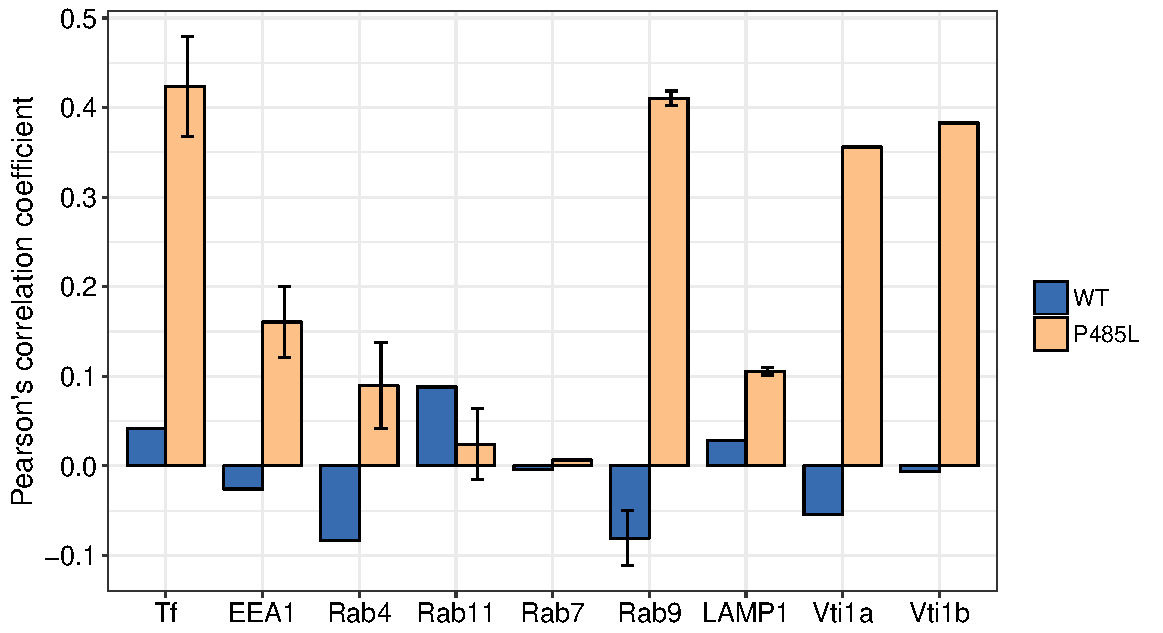
\includegraphics[scale=0.7]{Figures/coloc}
\caption{Colocalization coefficients for GLUT1 variants and intracellular markers.}
\vspace*{-3mm}
\small \justify
Pearson's thresholded coefficients (as implemented in the Imaris software) was determined for the indicated pairs of proteins. Two or three images from biological replicate experiments were evaluated for some of the colocalization analyses. Mean values were expressed with standard deviations of the mean.
\label{fig:coloc}
\end{figure}
%----------------------------------------------------------------------------------------
% Define some commands to keep the formatting separated from the content 
